% !TEX encoding   = UTF8
% !TEX spellcheck = ru_RU
% !TEX root = ../seminars.tex

%%===============================================
\chapter{Графические пользовательские интерфейсы}
%%===============================================

%%====================================
\section{Окно с кнопкой \texttt{Quit}}
%%====================================
Выполним упражнение~1 из~\textbookref{главы~16} учебника. Для~этого пронаследуем \code{My\_window} от~класса \code{Simple\_window} из~библиотеки \code{Graph\_lib}. Затем добавим по~аналогии с~кнопкой \code{Next} кнопку \code{Quit}, как показано на~рисунке~\ref{fig:mywindow}.

\begin{figure}[ht]
    {\centering
        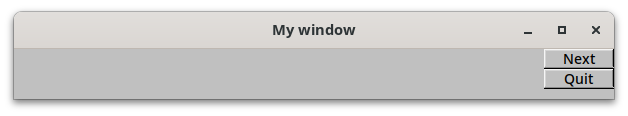
\includegraphics[width=0.6\textwidth]{images/my_window.png}

    }
    \caption{Простое окно \code{My\_window} с кнопкой \code{Quit}}
    \label{fig:mywindow}
\end{figure}

Из~документации к~библиотеке \name{FLTK} известно, что если все окна становятся скрытыми, то цикл обработки событий прекращает работу. То есть для~реализации функции \code{quit()} можно воспользоваться методом \code{hide()}.

\cppfile[firstline=11, lastline=30]{projects/ch16/chessboard/board.h}



%%=======================
\section{Шахматная доска}
%%=======================
Покажем, как можно создать клеточное поле и взаимодействовать с~ним на~примере упражнения~2 из~\textbookref{главы~16}. Эти идеи можно использовать для~создания практически любой игры с~клеточным полем: шашки, шахматы, сапёр, морской бой и другие.

\begin{figure}[ht]
    {\centering
        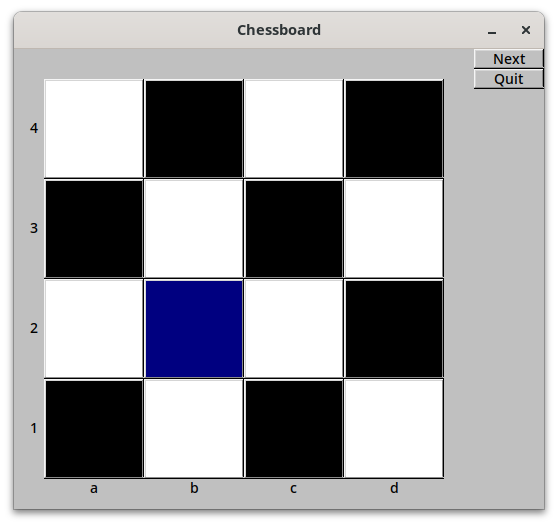
\includegraphics[width=0.5\textwidth]{images/chessboard.png}

    }
    \caption{Окно с шахматной доской \(4\times 4\)}
    \label{fig:chessboard}
\end{figure}

Размеры клеток и, соответственно, окна зафиксируем. Впоследствии, такое поведение можно изменить. Клетки представим квадратными кнопками и будем хранить их в~\code{Vector\_ref}. Метки строк и столбцов доски можно нарисовать при~помощи объектов \code{Marks}. Окно, согласно заданию, пронаследуем от~\code{My\_window} из~предыдущего упражнения.

\cppfile[firstline=32, lastline=60]{projects/ch16/chessboard/board.h}

Учитывая последующую доработку, код удобнее распределить между~несколькими файлами, как это предлагается в~таблице~\ref{tab:chessboard}.
\begin{table}[ht]
    {\centering\begin{tabular}{ll}
    \toprule
        \code{board.h}   & класс \code{Chessboard} для~шахматной доски, а также \code{My\_window} \\
        \code{board.cpp} & \\[0.5em]

        \code{cell.h}   & класс \code{Cell} для~шахматной клетки \\
        \code{cell.cpp} & \\[0.5em]

        \code{main.cpp} & \\
        \bottomrule
    \end{tabular}

    }
    \medskip
    \caption{Распределение кода <<шахматной доски>> между файлами}
    \label{tab:chessboard}
\end{table}

Конструктор задаёт размеры окна, создаёт клетки, располагая их в~соответствующих позициях, и рисует метки строк и столбцов доски. Зафиксировать размеры окна, чтобы пользователь не~смог его растягивать или сжимать, позволяет функция \code{size\_range()} "--- метод окна \name{FLTK}.

\cppfile[firstline=35, lastline=66]{projects/ch16/chessboard/board.cpp}

Цвет клетки (или тип) вычисляется на~основе номеров строки и столбца, определяющих её положение на~доске. Клетка в~левом нижнем углу имеет чёрный цвет. Обратим внимание, что клетки добавлялись в~линейный массив по~порядку в~соответствии с~направлением снизу вверх и слева направо, как принято в~шахматах.

\cppfile[firstline=7, lastline=13]{projects/ch16/chessboard/board.cpp}

Метки \code{Marks} допускают всего лишь один символ, поэтому мы используем ограничение \code{N\_max} для~максимального размера доски. Если потребуется вывести двузначные номера клеток, придётся разработать новый класс или добавить метки при~помощи неименованных объектов \code{Text}. А пока используем простую реализацию и пару вспомогательных функций:

\cppfile[firstline=15, lastline=33]{projects/ch16/chessboard/board.cpp}

\noindent Таким образом, получается вид, как на~рисунке~\ref{fig:chessboard}.

В~функцию-обработчик нажатия на~кнопку-клетку добавим простую логику самой шахматной доски. Мы можем выделить любую клетку; переместить выделение, выбрав другую клетку; или снять выделение, нажав на~выделенную клетку повторно:

\cppfile[firstline=68, lastline=90]{projects/ch16/chessboard/board.cpp}

\noindent\textbf{NB!} Если в~отображении виджета что-то изменилось, то, скорее всего, потребуется перерисовать его вручную. Для~этого используйте \code{Fl::redraw()}.

Теперь посмотрим реализацию клетки шахматной доски:

\cppfile[firstline=8, lastline=32]{projects/ch16/chessboard/cell.h}

Реализация методов проста и не~требует дополнительных пояснений, кроме того, что \code{pw} "--- это защищённый член класса \code{Graph\_lib::Widget}, связанный с~реальным графическим виджетом из~\name{FLTK}.
\enlargethispage{0.5\baselineskip}

\cppfile[firstline=5, lastline=32]{projects/ch16/chessboard/cell.cpp}

Теперь настало время собрать и запустить программу целиком. Для~этого добавьте необходимые заголовки и функцию \code{main()}, просто создающую окно \code{Checkerboard} и запускающую цикл обработки событий:

\cppfile[firstline=17, lastline=18]{projects/ch16/chessboard/main.cpp}



\clearpage
%%===============================
\section{Добавление фигур. Шашки}
%%===============================

\begin{figure}[ht]
    {\centering
        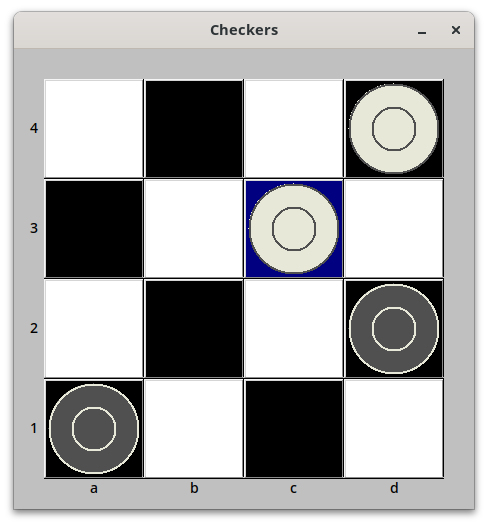
\includegraphics[width=0.5\textwidth]{images/checkers.png}

    }
    \caption{Шахматная доска \(4\times 4\) с~шашками}
    \label{fig:checkers}
\end{figure}

\todo{Описание будет добавлено позже.}



%%================
\WhatToReadSection
%%================
\textcite{Stroustrup:2016:ru}: \textbf{глава~17}



%%===============
\ExercisesSection
%%===============
\begin{exercise}
\item Выполните упражнения из~\textbookref{главы~16} учебника.

\end{exercise}
